\part{Connection}
\label{connection}

The protocol is divided to two mutually independent layers. That structure separates connection and data transfer from protocol sense and data representation. Protocol layers are illustrated on figure \ref{connection.pictures.protocol_layers}.


\begin{figure}[h]
  \centering
  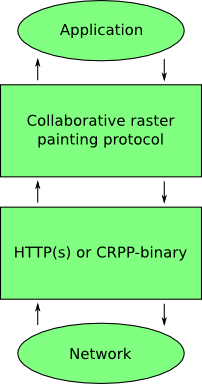
\includegraphics[width=0.30\textwidth]{diagrams/protocol_layers.png}
  \caption{Protocol layers diagram}
  \label{connection.pictures.protocol_layers}
\end{figure}

Top layer interchanges monolithic data chunks with bottom layer. Bottom layer deliver this data to the up layer on other side of connection. Top layer is described on \ref{up_layer} and bottom layer is described on \ref{down_layer}.

\chapter{Data types}
\label{connection.data_types}

If it is not say otherwise all integers are unsigned.

\section{Unsigned integers}
\label{connection.data_types.unsigned_integer}

Every bit of value $1$ represents number $2^{p}$, where $p$ is bit position in big-endian notation. $0$ bits represent $0$. The value of integer is than sum of all bits. Equation \ref{equation.unsigned-integers-sum} is specifying number value.

\begin{equation}
\label{connection.equations.unsigned_integer}
\sum_{p = 0}^{n - 1} b_p 2^p
\end{equation}

$p$ is bit position (the last has value $0$, than value is increasing by step $1$), $n$ is count of bits representing the number, $b_p$ is bit value($0$ or $1$) on position $p$.

For example sequence $00001010$ has value $10$ ($2^1 + 2^3$).

\section{Signed integers}

Hodnota znaménkového celého čísla je součet čísel $a$ and $b$ (it is ${value} = a + b$). 

Hodnotu proměnné $a$ uručje vzorec $a = -2^{n - 1} \cdot f$, kde $n$ je počet bitů reprezentujících číslo a $f$ první bit ($0$ or $1$).

Hodnotu promměné $b$ určuje vzorec \ref{connection.equations.unsigned_integer} přičemž první bit není do vzorce vložen. Například posloupnost $10011$ by měla hodnotu $b = 2^0 + 2^1$ (není zahrnut první bit $1$).

Příklad: číslo reprezentované bity $1011$ má hodnotu $-5$ ($a = -2^3 \cdot 1 = -8$, $b = 2^1 + 2^0 = 3$, $a + b = -8 + 3 = -5$).

\section{Floating point numbers}

Real number are used in meaning of standard IEEE 754 with 32 bites.

\section{Logical value (booleans)} 

Logical values (boolean) are represented by one byte, where full zeros ($00000000$) means \emph{false} and value one ($00000001$) represents \emph{true}. Every other value is considered as invalid.

\section{Strings}

If it is not specified otherwise text (characters string) is coded by UTF-8 (Unicode). In several cases ASCII is use instead. Protocol is case sensitive. 

\section{Image}
\label{connection.data_types.image}

Every image is represented as binary data of PNG \url{http://www.w3.org/Graphics/PNG/}. PNG image is specified by standard ISO/IEC 15948:2003 (E), see \url{http://www.w3.org/TR/PNG/}.

In all cased ARGB PNG is used (four 8 bites channels: alpha -- transparency, red, green, blue), that is 32 deep.